% -- Encoding UTF-8 without BOM
% -- XeLaTeX => PDF (BIBER)

\documentclass[espanol]{cv-style}     % Add 'print' as an option into the square bracket to remove colours from this template for printing. 
                                      % Add 'espanol' as an option into the square bracket to change the date format of the Last Updated Text
%\setdefaultlanguage{spanish}
%\sethyphenation[variant=spanish]{}{}  % Add words between the {} to avoid them to be cut 

\usepackage{graphicx}

\begin{document}

\header{Jesús Adolfo }{Abano Ferrara}
\lastupdated

%----------------------------------------------------------------------------------------
% SIDEBAR SECTION  -- In the aside, each new line forces a line break
%----------------------------------------------------------------------------------------
\begin{aside}
\section{-}
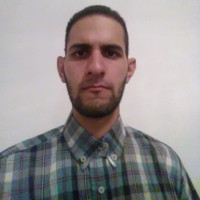
\includegraphics[width=4cm]{perfileLinkedin.jpeg}
%
\section{datos personales}
Jesús Adolfo Abano Ferrara
25 años, venezolano
C.I. 24540196
%
\section{contacto}
(+58) 424 3159364
~
jaabanof@gmail.com
~
Maracay, Edo. Aragua.
%
\section{idiomas}
Español (Lengua materna),
Inglés (Básico)
%
% \section{lenguajes de programación}
% {\color{red} $\varheartsuit$} Python, C, C++, Haskell, Assembler, Bash/Zsh Scripting, Java
% %
\section{desarrollo web}
Flask, Bootstrap, HTML5, CSS3, JavaScript
% %
% \section{tecnologías miscelaneas}
% {\color{red} $\varheartsuit$} OpenSource, Gentoo/Ubuntu/Debian y otros Linux, Scrapy Crawling y Scraping Framework, NTKL (Natural Language Toolkit), RabbitMQ, MemCached, SVN/GIT Source Version Control, MySQL/PostgreSQL/ LiteSQL/MongoDB DataBases, Latex
%
\end{aside}
%----------------------------------------------------------------------------------------
% RESUMEN SECTION
%----------------------------------------------------------------------------------------
\vspace{0.2cm}
\section{Resumen}
  \vspace{-0.2cm}
Soy Ingeniero en Telecomunicaciones, con conocimientos en las áreas de señales y sistemas, electromagnetismo, antenas y propagación. Conocimiento en redes informáticas y configuración básica de equipos con software \textbf{Cisco IOS} y \textbf{MikroTik RouterOS}. Experiencia en el diseño de aplicaciones web con el framework \textbf{Flask} y programación en general con \textbf{Python}. Manejo de sistemas operativos \textbf{Windows} y \textbf{Linux}. Sistema de control de versiones \textbf{Git}. Capaz de aprender de forma constante y responsable, también soy proactivo y con capacidad de adaptación a los cambios. Siempre en búsqueda de potenciar mis habilidades y adquirir nuevos conocimientos.
%----------------------------------------------------------------------------------------
% WORK EXPERIENCE SECTION
%----------------------------------------------------------------------------------------
% \section{experiencia}
%   \vspace{-0.2cm}
% \begin{entrylist}
% %------------------------------------------------
%----------------------------------------------------------------------------------------
% EDUCATION SECTION
%----------------------------------------------------------------------------------------
\section{Educación}
  \vspace{-0.2cm}
\begin{entrylist}
%------------------------------------------------
\entry
{\scalebox{.8}[1.0]{2011--2019}}
{Ingeniería en Telecomunicaciones}
{Universidad de Carabobo, UC}
{\textbf{}
\\
\small{Profesional de la ingeniería que puede desempeñarse en las diferentes empresas de telecomunicaciones en las actividades de instalación, operación y mantenimiento de equipos de telecomunicaciones, así como gestión de sistemas y servicios de telecomunicaciones. Capaz de resolver problemas y gerenciar proyectos de diversa índole y alcance, en los que las tecnologías de la información y las telecomunicaciones son un elemento clave.}}
%------------------------------------------------
\end{entrylist}
%----------------------------------------------------------------------------------------
% AWARDS SECTION
%----------------------------------------------------------------------------------------
\section{Cursos}
  \vspace{-0.2cm}
\begin{entrylist}
%------------------------------------------------
\entry
{\scalebox{.8}[1.0]{2018}}
{CCNA Routing and Switching: Introducción a redes}
{Emprevet S.A.}
{Capacitado para explicar las tecnologías de red, cómo los dispositivos tienen acceso a los recursos de red local y remota, la forma en que funciona el switching en una red de pequeña o mediana empresa, diseñar un esquema de direccionamiento IP para proporcionar conectividad a una red de pequeña o mediana empresa e implementar la conectividad de red básica entre dispositivos.}
%------------------------------------------------
\entry
{\scalebox{.8}[1.0]{2019}}
{Redes neuronales y aprendizaje profundo}
{Coursera}
{Capacitado para comprender las principales tendencias tecnológicas que impulsan el aprendizaje profundo. Poder construir, entrenar y aplicar redes neuronales profundas totalmente conectadas. Comprender los parámetros clave en la arquitectura de una red neuronal.}
%------------------------------------------------
\entry
{\scalebox{.8}[1.0]{2019}}
{Desarrollo Web Online}
{Platzi}
{Capacitado para crear sitios web estáticos con HTML y CSS3, dominar HTML y su estructura, aplicar estilos con CSS y definir la arquitectura de un sitio web.}
%------------------------------------------------


\end{entrylist}
  \vspace{-0.2cm}
%----------------------------------------------------------------------------------------
% INTERESTS SECTION
%----------------------------------------------------------------------------------------3
\section{Intereses}
  \vspace{-0.2cm}
% \textbf{Back-end.} Sectores de análisis de datos y categorización (Natural Language Processing, Machine Learning); optimización de procesos; mantenimiento de servidores y bases de datos; seguridad informática.
\begin{itemize}
    \item Redes informáticas.
    \item Telefonía.
    \item Programación.
    \item Inteligencia artificial.
    \item Telecomunicaciones en general.
\end{itemize}
%----------------------------------------------------------------------------------------
\end{document}
